\section{Metodología}

El presente trabajo se desarrolló como una extensión y comparación del estudio realizado por Quintero y Botía et al. \cite{ref10} sobre la subrogación de modelos para el control predictivo de un proceso de destilación extractiva. La metodología se estructuró en dos fases principales: $(i)$ la replicación y verificación de la base metodológica establecida en dicho trabajo, que incluye el caso de estudio, las simulaciones rigurosas y la generación de datos dinámicos; y $(ii)$ la implementación y evaluación de nuevas estrategias de subrogación orientadas al control. En la primera fase se utilizó el mismo caso de estudio correspondiente a la separación de una mezcla azeotrópica metanol-acetona mediante destilación extractiva con dimetilsulfóxido (DMSO) como agente separador. Inicialmente, se verificó el correcto funcionamiento del modelo del proceso en estado estacionario en Aspen Plus. Posteriormente, el proceso fue llevado a un entorno dinámico mediante Aspen Plus Dynamics, donde se implementó la estructura de control regulatorio necesaria para garantizar la estabilidad hidráulica del sistema durante la operación. 

Una vez estabilizado el proceso en el entorno dinámico, se realizaron pruebas de escalón en las variables manipuladas del sistema, correspondientes al calor de rehervidor y la relación de reflujo en cada columna ($Q_{R,T-101}$, $Q_{R,T-102}$, $RR_{T-101}$ y $RR_{T-102}$), mientras se monitoreó la respuesta de las variables controladas asociadas a la pureza de los productos, representadas por las temperaturas en etapas específicas de las columnas ($T_{36,T-101}$ y $T_{8,T-102})$, para obtener datos dinámicos representativos del comportamiento del sistema frente a perturbaciones.

Estos datos fueron posteriormente utilizados para la construcción de modelos subrogados capaces de aproximar el comportamiento dinámico del modelo riguroso. En el trabajo original, la subrogación del sistema se realizó mediante representaciones en espacio de estados (SS). En el presente estudio, este método de subrogación se mantiene como referencia y se implementan adicionalmente modelos ARX y ARMAX con el objetivo de comparar el desempeño de diferentes estrategias de subrogación orientadas al control. Los modelos obtenidos fueron evaluados mediante métricas estadísticas de ajuste y posteriormente integrados en un esquema de control predictivo basado en modelo (MPC) mediante una co-simulación entre Aspen Plus Dynamics y MATLAB®–Simulink®, lo que permitió analizar su desempeño frente a perturbaciones en las corrientes de alimentación del proceso.

\begin{figure}[h!]
    \centering
    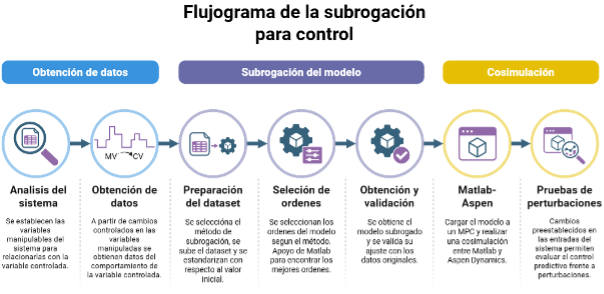
\includegraphics[width=0.6\textwidth]{figures/ProcesoControl.png}
    \caption{Flujo del proceso de subrogación de modelos para el control predictivo}
    \label{fig:ProcesoControl}
\end{figure}

\subsection{Software empleado}

Para el desarrollo de las simulaciones del proceso se empleó la suite aspenONE® de Aspen Technology Inc. (versión 11), específicamente los programas Aspen Plus V11 y Aspen Plus Dynamics V11, con el objetivo de simular el proceso tanto en estado estacionario como en régimen dinámico. Los datos generados durante la simulación dinámica fueron posteriormente exportados al entorno de MATLAB® y Simulink® R2025b de MathWorks Inc. En este entorno se realizaron las tareas de procesamiento de datos, la identificación de modelos subrogados y la implementación de los esquemas de control predictivo basados en modelo (MPC). Para la identificación de los modelos ARX y ARMAX se empleó el System Identification Toolbox de MATLAB®, el cual permite estimar modelos dinámicos a partir de datos de entrada-salida obtenidos del proceso. Por otra parte, el esquema de control MPC se implementó mediante el Model Predictive Control Toolbox, lo que permitió integrar directamente los modelos identificados en el controlador y evaluar su desempeño en el entorno de co-simulación con Aspen Plus Dynamics.



\subsection{Caso de estudio y simulación rigurosa}

Con el fin de establecer una base de comparación consistente, se adoptó el mismo caso de estudio y el modelo riguroso desarrollado por Quintero y Botía et al. \cite{ref10} correspondiente a un proceso de destilación extractiva para la separación de una mezcla azeotrópica de metanol y acetona.

\subsubsection{Descripción del proceso}

El proceso consiste en la separación de una mezcla azeotrópica de metanol-acetona mediante destilación extractiva utilizando dimetilsulfóxido (DMSO) como agente separador. La configuración del sistema está compuesta por dos columnas de destilación acopladas: una columna extractiva $T-101$ y una columna de recuperación de solvente $T-102$. En la columna extractiva $T-101$ se introduce la mezcla azeotrópica junto con el solvente DMSO, el cual modifica el equilibrio vapor-líquido del sistema y permite romper el azeótropo. Como resultado, la acetona se obtiene en el destilado mientras que la corriente de fondo contiene metanol y solvente. Esta corriente se envía posteriormente a la columna $T-102$, donde se realiza la recuperación del solvente mediante destilación, obteniéndose metanol en el destilado y DMSO en el fondo para su recirculación al proceso. El modelo del proceso se implementó inicialmente en Aspen Plus para verificar la consistencia de las condiciones operativas en estado estacionario antes de su análisis dinámico.

\subsubsection{Esquema de control regulatorio}

Para garantizar la estabilidad hidráulica y operativa del sistema durante las simulaciones dinámicas, se implementó un esquema de control regulatorio basado en controladores de retroalimentación proporcional-integral (PI). 
El sistema de control incluye lazos de control de nivel en los tanques de condensadores y rehervidores de ambas columnas, así como lazos de control de presión en cada columna de destilación. Estos lazos permiten mantener condiciones de operación estables y evitar problemas operativos tales como sobrellenado de equipos o variaciones de presión dentro del sistema. La sintonización de los controladores PI se realizó mediante el método de Tyreus-Luyben, el cual se basa en la determinación de la ganancia y el período últimos del sistema para establecer los parámetros de control adecuados. Los valores finales de sintonización corresponden a los reportados por Quintero y Botía et al. \cite{ref10}. Una vez implementado el esquema de control, se realizó una prueba de estabilidad del sistema para verificar su correcto funcionamiento. Para esta prueba se aplicó una perturbación tipo escalón correspondiente a un incremento del 15\% en el flujo molar de la corriente de alimentación azeotrópica respecto a su valor nominal. Los resultados obtenidos confirmaron que el sistema de control regulatorio permite mantener la estabilidad hidráulica del proceso, lo que constituye una base adecuada para el análisis dinámico posterior.

\subsubsection{Generación de datos dinámicos mediante pruebas de escalón}

Para obtener los datos necesarios para la identificación de modelos subrogados se realizaron pruebas de escalón (step tests) en la simulación dinámica del proceso utilizando Aspen Plus Dynamics. Estas pruebas consisten en aplicar cambios escalón en las variables manipuladas del proceso y registrar la respuesta dinámica de las variables de interés, con el propósito de excitar la dinámica del sistema y generar información suficiente para la identificación de modelos dinámicos.

En el contexto de la subrogación orientada al control, las variables manipuladas consideradas fueron la potencia de los rehervidores y la razón de reflujo de cada columna. Debido a que la medición directa de fracciones molares en procesos industriales continuos puede resultar costosa o difícil de implementar, se seleccionaron las temperaturas de etapa como variables controladas, dado que presentan una fuerte correlación con la pureza de los productos. En particular, se seleccionaron la temperatura de la etapa 36 para la columna $T-101$ y la temperatura de la etapa 8 para la columna $T-102$, debido a su alta sensibilidad frente a cambios en las condiciones operativas.

Durante el análisis de los datos obtenidos se observó la presencia de pequeñas variaciones residuales en las señales de temperatura que no son completamente explicadas por los cambios escalón aplicados. Estas variaciones pueden interpretarse como ruido en los datos, asociado principalmente aerrores de modelado y a la capacidad limitada de los modelos subrogados para reproducir completamente la dinámica del sistema, así como a efectos numéricos inherentes a la discretización temporal y a los algoritmos de integración empleados en la simulación dinámica. Este comportamiento resulta relevante para la identificación de modelos subrogados, particularmente en estructuras como los modelos ARX y ARMAX, en los cuales el término de ruido representa dinámicas no modeladas y errores de aproximación inherentes al proceso de identificación


\subsection{Subrogación de modelos}

La subrogación del proceso se realizó con el objetivo de construir modelos dinámicos simplificados capaces de reproducir el comportamiento del modelo riguroso y que puedan ser utilizados dentro de esquemas de control predictivo basado en modelo. En el trabajo original de Quintero y Botía et al. \cite{ref10}, la subrogación se realizó mediante representaciones en espacio de estados. En el presente estudio, dicho modelo se mantiene como referencia o línea base para la comparación, y se implementan adicionalmente modelos de tipo ARX y ARMAX con el fin de evaluar su capacidad para representar la dinámica del proceso.

\subsubsection{Preprocesamiento de datos}

Antes de identificar los modelos, todas las variables de entrada y salida se transformaron en desviaciones respecto a su valor nominal de operación. Esta transformación permite centrar el análisis en la dinámica del proceso alrededor del punto de operación. La desviación de cada variable se calculó mediante:

\begin{equation}
X_{desv} = \frac{(X-X_{nominal})}{X_{nominal}}
\label{eq:Desviacion}
\end{equation}

\subsubsection{Identificación de modelos subrogados}

La identificación de los modelos subrogados se realizó en el entorno MATLAB® R2025b, empleando el System Identification Toolbox, a partir de los datos obtenidos de las simulaciones dinámicas del proceso. En primer lugar, se consideró como referencia el modelo en espacio de estados desarrollado en el trabajo previo. Posteriormente, se identificaron modelos de tipo ARX y ARMAX con el objetivo de evaluar su capacidad para aproximar la dinámica del proceso mediante estructuras lineales discretas. Para los modelos ARX se llevó a cabo un barrido sistemático de órdenes utilizando las funciones arxstruc y selstruc del toolbox, las cuales permiten explorar automáticamente distintas combinaciones de parámetros autorregresivos y exógenos. En este contexto, los términos autorregresivos corresponden a valores pasados de la variable de salida del sistema (temperatura de etapa), mientras que los términos exógenos representan la influencia de las variables de entrada del proceso, en este caso la potencia del rehervidor y la razón de reflujo de cada columna. Una vez determinada la estructura ARX más adecuada, esta se utilizó como base para la identificación de modelos ARMAX, variando el orden asociado al polinomio de ruido (nc) y estimando los parámetros del modelo mediante las rutinas de identificación disponibles en el toolbox. Para cada valor de nc, se generó un modelo candidato y se evaluó su desempeño mediante simulación frente a los datos originales. El desempeño de cada modelo, para cada columna del proceso ($T-101$ y $T-102$), se evaluó mediante el coeficiente de determinación (R²) y el error cuadrático medio (RMSE) entre las salidas del modelo y los datos generados por el modelo riguroso. Estos indicadores permitieron seleccionar las estructuras con mejor capacidad predictiva para su posterior implementación en el esquema de control predictivo basado en modelo.

\subsubsection{Métricas de evaluación}

Para evaluar la capacidad de los modelos subrogados de reproducir la dinámica del proceso se emplearon métricas estadísticas de ajuste. En particular, se calcularon el coeficiente de determinación $R^2$ y  la media cuadrática del error (RECM), los cuales permiten cuantificar la calidad del ajuste entre las predicciones del modelo y los datos obtenidos de la simulación rigurosa. Las métricas se calcularon según las ecuaciones \ref{eq:RECM} y \ref{eq:R2}:

\begin{equation}
RECM= \sqrt[2]{\frac{\sum_{n=1}^N (y_n - \hat{y}_n)^2}{N}}
\label{eq:RECM}
\end{equation}

\begin{equation}
R^2 = 1 - \frac{\sum_{n=1}^N (y_n - \hat{y}_n)^2}{\sum_{n=1}^N (y_n - \bar{y})^2}
\label{eq:R2}
\end{equation}

\subsection{Implementación del control MPC y co-simulación}

Con el fin de evaluar el desempeño de los modelos subrogados dentro de un entorno de control, se implementó un esquema de MPC mediante una co-simulación entre Aspen Plus Dynamics y MATLAB®–Simulink®. En este esquema, la simulación dinámica del proceso se ejecuta en Aspen Plus Dynamics, mientras que el controlador MPC se implementa en Simulink. La comunicación entre ambos entornos permite que el controlador utilice los modelos subrogados para calcular las acciones de control en cada instante.Las variables manipuladas consideradas fueron la potencia de los rehervidores y la razón de reflujo de las columnas, mientras que las variables controladas correspondieron a las temperaturas de etapa seleccionadas para cada columna. Para evaluar el desempeño del controlador se aplicaron perturbaciones de tipo escalón en los flujos de alimentación del proceso durante un horizonte dinámico de simulación de 100 horas. El desempeño del sistema de control se evaluó en términos del error relativo respecto al valor nominal de la variable controlada, del tiempo de estabilización del sistema y del esfuerzo de control requerido para mantener la operación estable.

\subsubsection{Formulación del problema de optimización MPC}

En cada instante de control k, el controlador MPC resuelve un problema de optimización utilizando un problema de programación cuadrática (QP). Este tiene un vector de decisión $z_k$ que define la secuencia futura de acciones de control frente a las variables manipuladas:

\begin{equation}
z_k^T=[u(k|k)^T u(k+1|k)^T \cdots u(k+p-1|k)^T, \epsilon_k )]
\label{eq:Vectorzk}
\end{equation}

\begin{equation}
\min_{z_k} J(z_k) = J_y(z_k) + J_u(z_k) + J_{\Delta u}(z_k) + J_{\epsilon}(z_k)
\label{eq:OptimizationProblem}
\end{equation}
    
Dentro del vector, se optimizan dichas acciones a lo largo del horizonte de predicción p, al mismo tiempo que $\epsilon_k$ penaliza las violaciones de las restricciones. El MPC realiza la acción de la ecuación \ref{eq:OptimizationProblem}, minimizando una función de costo resultante de la suma de cuatro términos. El primer termino $J_y$, formulado en la ecuación \ref{eq:Jy}, compara el error entre las salidas propuestas por los metamodelos con su referencia a lo largo del horizonte, mientras que $J_u$, de la ecuación \ref{eq:Ju}, penaliza las desviaciones de las dos variables manipuladas con respecto al valor en estado estable. Por el otro lado, el término $J_{\Delta u}$, expuesto en la ecuación \ref{eq:Jdeltau}, compara los cambios en las variables manipuladas consecutivas para evitar cambios bruscos. Por último, $J_{\epsilon}$ penaliza la variable de relajación asociada a posibles violaciones de restricciones, garantizando que estas solo ocurran cuando sea estrictamente necesario \cite{ref24}.

\begin{equation}
J_y (z_k )=\sum_{j=1}^{n_y}\sum_{i=1}^{p}\left\{\frac{w_{i,j}^y}{s_j^y} [r_j (k+i|k)-y_j (k+i|k)]\right\}^2 
\label{eq:Jy}
\end{equation}

\begin{equation}
J_u (z_k )=\sum_{j=1}^{n_u}\sum_{i=1}^{p-1}\left\{\frac{w_{i,j}^u}{s_j^u} [u_j (k+i|k)-u_{j,target} (k+i|k)]\right\}^2
\label{eq:Ju}
\end{equation}

\begin{equation}
J_{\Delta u} (z_k )=\sum_{j=1}^{n_u}\sum_{i=1}^{p-1}\left\{\frac{w_{i,j}^{\Delta u}}{s_j^u} [u_j (k+i|k)-u_j (k+i-1|k)]\right\}^2     
\label{eq:Jdeltau}
\end{equation}

\begin{equation}
J_{\varepsilon} (z_k )=\rho_{\varepsilon} \varepsilon_k^2 
\label{eq:Jepsilon}
\end{equation}

En el contexto del estudio realizado, los modelos subrogados SS, ARX y ARMAX son los responsables del cálculo de las salidas predichas y   $(k+i|k)$, además de proporcionar la relación dinámica entre las variables manipuladas futuras $u(k+i|k)$ y el comportamiento esperado del proceso; permitiendo así que el optimizador evalúe el impacto de cada posible secuencia de control sobre el desempeño futuro del sistema.

\subsubsection{Integración con Aspen Plus Dynamics}

La co-simulación entre Simulink y Aspen Plus Dynamics se realiza mediante el intercambio de señales de entrada y salida en cada intervalo de muestreo, donde Aspen envía a Simulink las mediciones actuales de las variables controladas (temperaturas de etapa) y el controlador MPC calcula las acciones de control, las cuales son enviadas de regreso a Aspen como ajustes en la potencia de los rehervidores y en la razón de reflujo, permitiendo así cerrar el lazo de control y considerar de forma dinámica la influencia de perturbaciones externas en el proceso. 

\subsubsection{Evaluación del desempeño del controlador}
\label{sec:criterios}

Para cuantificar la efectividad del esquema de control implementado, se evaluó el desempeño del sistema mediante un conjunto de métricas que permiten analizar la calidad del seguimiento de referencia, la rapidez de respuesta del sistema y el esfuerzo requerido por las variables manipuladas. El error relativo de seguimiento permite cuantificar la diferencia entre el valor de la variable controlada y su valor de referencia a lo largo del tiempo. Este indicador se calcula mediante la siguiente expresión:

\begin{equation}
e_{rel}(t)= \frac{|Y(t)-Y_{ref} (t)|}{Y_{ref} (t)}
\label{eq:ErrorRelativo}
\end{equation}

El tiempo de estabilización se define como el tiempo requerido para que las variables controladas ingresen y permanezcan dentro de una banda de tolerancia de ±2\% respecto a su valor nominal después de la aplicación de una perturbación. Este indicador permite evaluar la rapidez con la que el sistema recupera condiciones estables de operación. Además, para evaluar con mayor precisión la calidad del control, se utilizaron las siguientes métricas de error integral.

El criterio de la integral del valor absoluto del error (IAE) mide el error absoluto acumulado a lo largo del tiempo y se calcula como:

\begin{equation}
\text{IAE} = \int_0^{\infty} |e(t)| \, dt
\label{eq:IAE}
\end{equation}

El criterio de la integral del error cuadrático mide el error cuadrático acumulado, penalizando los errores de mayor magnitud:

\begin{equation}
\text{ISE} = \int_0^{\infty} e^2(t) \, dt
\label{eq:ISE}
\end{equation}

Por otro lado, el criterio de la integral del valor absoluto del error multiplicado por el tiempo (ITAE) pondera los errores con el tiempo, favoreciendo la penalización de los errores que persisten durante períodos prolongados:

\begin{equation}
\text{ITAE} = \int_0^{\infty} t|e(t)| \, dt
\label{eq:ITAE}
\end{equation}

Finalmente, la integral del error cuadrático multiplicado por el tiempo (ITSE) es una métrica análoga a la ITAE, pero incorpora el error al cuadrado, lo que incrementa la penalización de los errores de mayor magnitud y duración:

\begin{equation}
\text{ITSE} = \int_0^{\infty} t e^2(t) \, dt
\label{eq:ITSE}
\end{equation}

Estas métricas de error integral permiten una evaluación más completa del desempeño del controlador, ya que cuantifican tanto la magnitud de los errores como su persistencia en el tiempo \cite{ref25}. Los resultados obtenidos con estas métricas permitieron comparar la capacidad de los distintos modelos subrogados para mantener la estabilidad del proceso, minimizar el error de seguimiento y reducir el esfuerzo de control requerido, proporcionando así una evaluación cuantitativa del desempeño de cada estrategia de modelado dentro del esquema de control predictivo basado en modelo.
